\section{Test Description}

After finishing the first version of our own negotiation agent, we were provided with the negotiation agents of other groups and their domains. We decided to do a comprehensive set of tests in the genius Tournament environment. 10 Tournaments were ran, for every opponent-profile combination of three parties per tournament, resulting in 2\textsuperscript{3} = 8 sessions per tournament. All opponents were tested in their own domain, with the following exceptions:

\begin{itemize}
	\item Opponent 9 was not tested, because we were unable to get the agent running. 
	\item Opponent 10 was tested on the domain of Opponent 12, because the domain of Opponent 10 was missing.
\end{itemize}

We were unable to determine which domain, provided by Opponent 2, was the cooperative, moderate and competitive domain, so we made the alphabetical assumption of \textit{Dinner}, \textit{Sporthal} and \textit{Politics} respectively. \\

We also note that sessions were only counted when an agreement was reached as shown in Figure \ref{fig:18_agreements} and \ref{fig:180_agreements}. This resulted in less data for Opponent 2, 6, 7 and 10, specifically for the variables: Distance to Pareto, Distance to Nash, Social Welfare, and the Utilities.

\begin{figure}[!htb]
	\minipage{0.49\textwidth}
	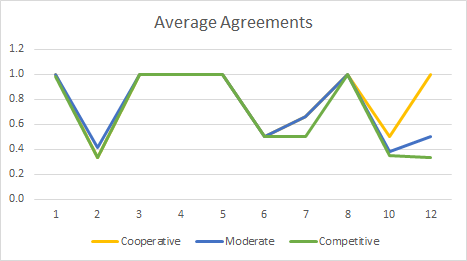
\includegraphics[width=\linewidth]{pre/18_agreements}
	\caption{18 Rounds per Opponent}
	\label{fig:18_agreements}
	\endminipage\hfill
	\minipage{0.49\textwidth}
	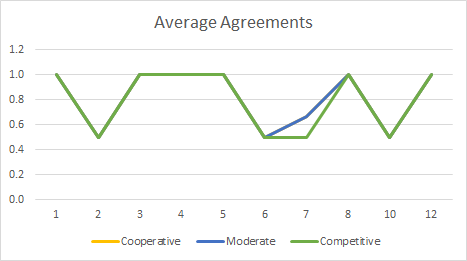
\includegraphics[width=\linewidth]{pre/180_agreements}
	\caption{180 Rounds per Opponent}
	\label{fig:180_agreements}
	\endminipage\hfill
\end{figure}

These tests were done twice, for both 18 and 180 maximal tournament rounds.
All results were then averaged over all sessions and domain types, ignoring the sessions with the following agent composition: n/n/n and 11/11/11. All these combined test resulted in a dataset of a whopping (60 $\cdot$ 30 $\cdot$ 2 =) 3600 sessions.